\begin{frame}
	\frametitle{Introduction}
	Actually two widely used techniques to store information:\\ \vspace{5mm}
	\begin{itemize}
	\item HDD (hard disc drives) is slower 
	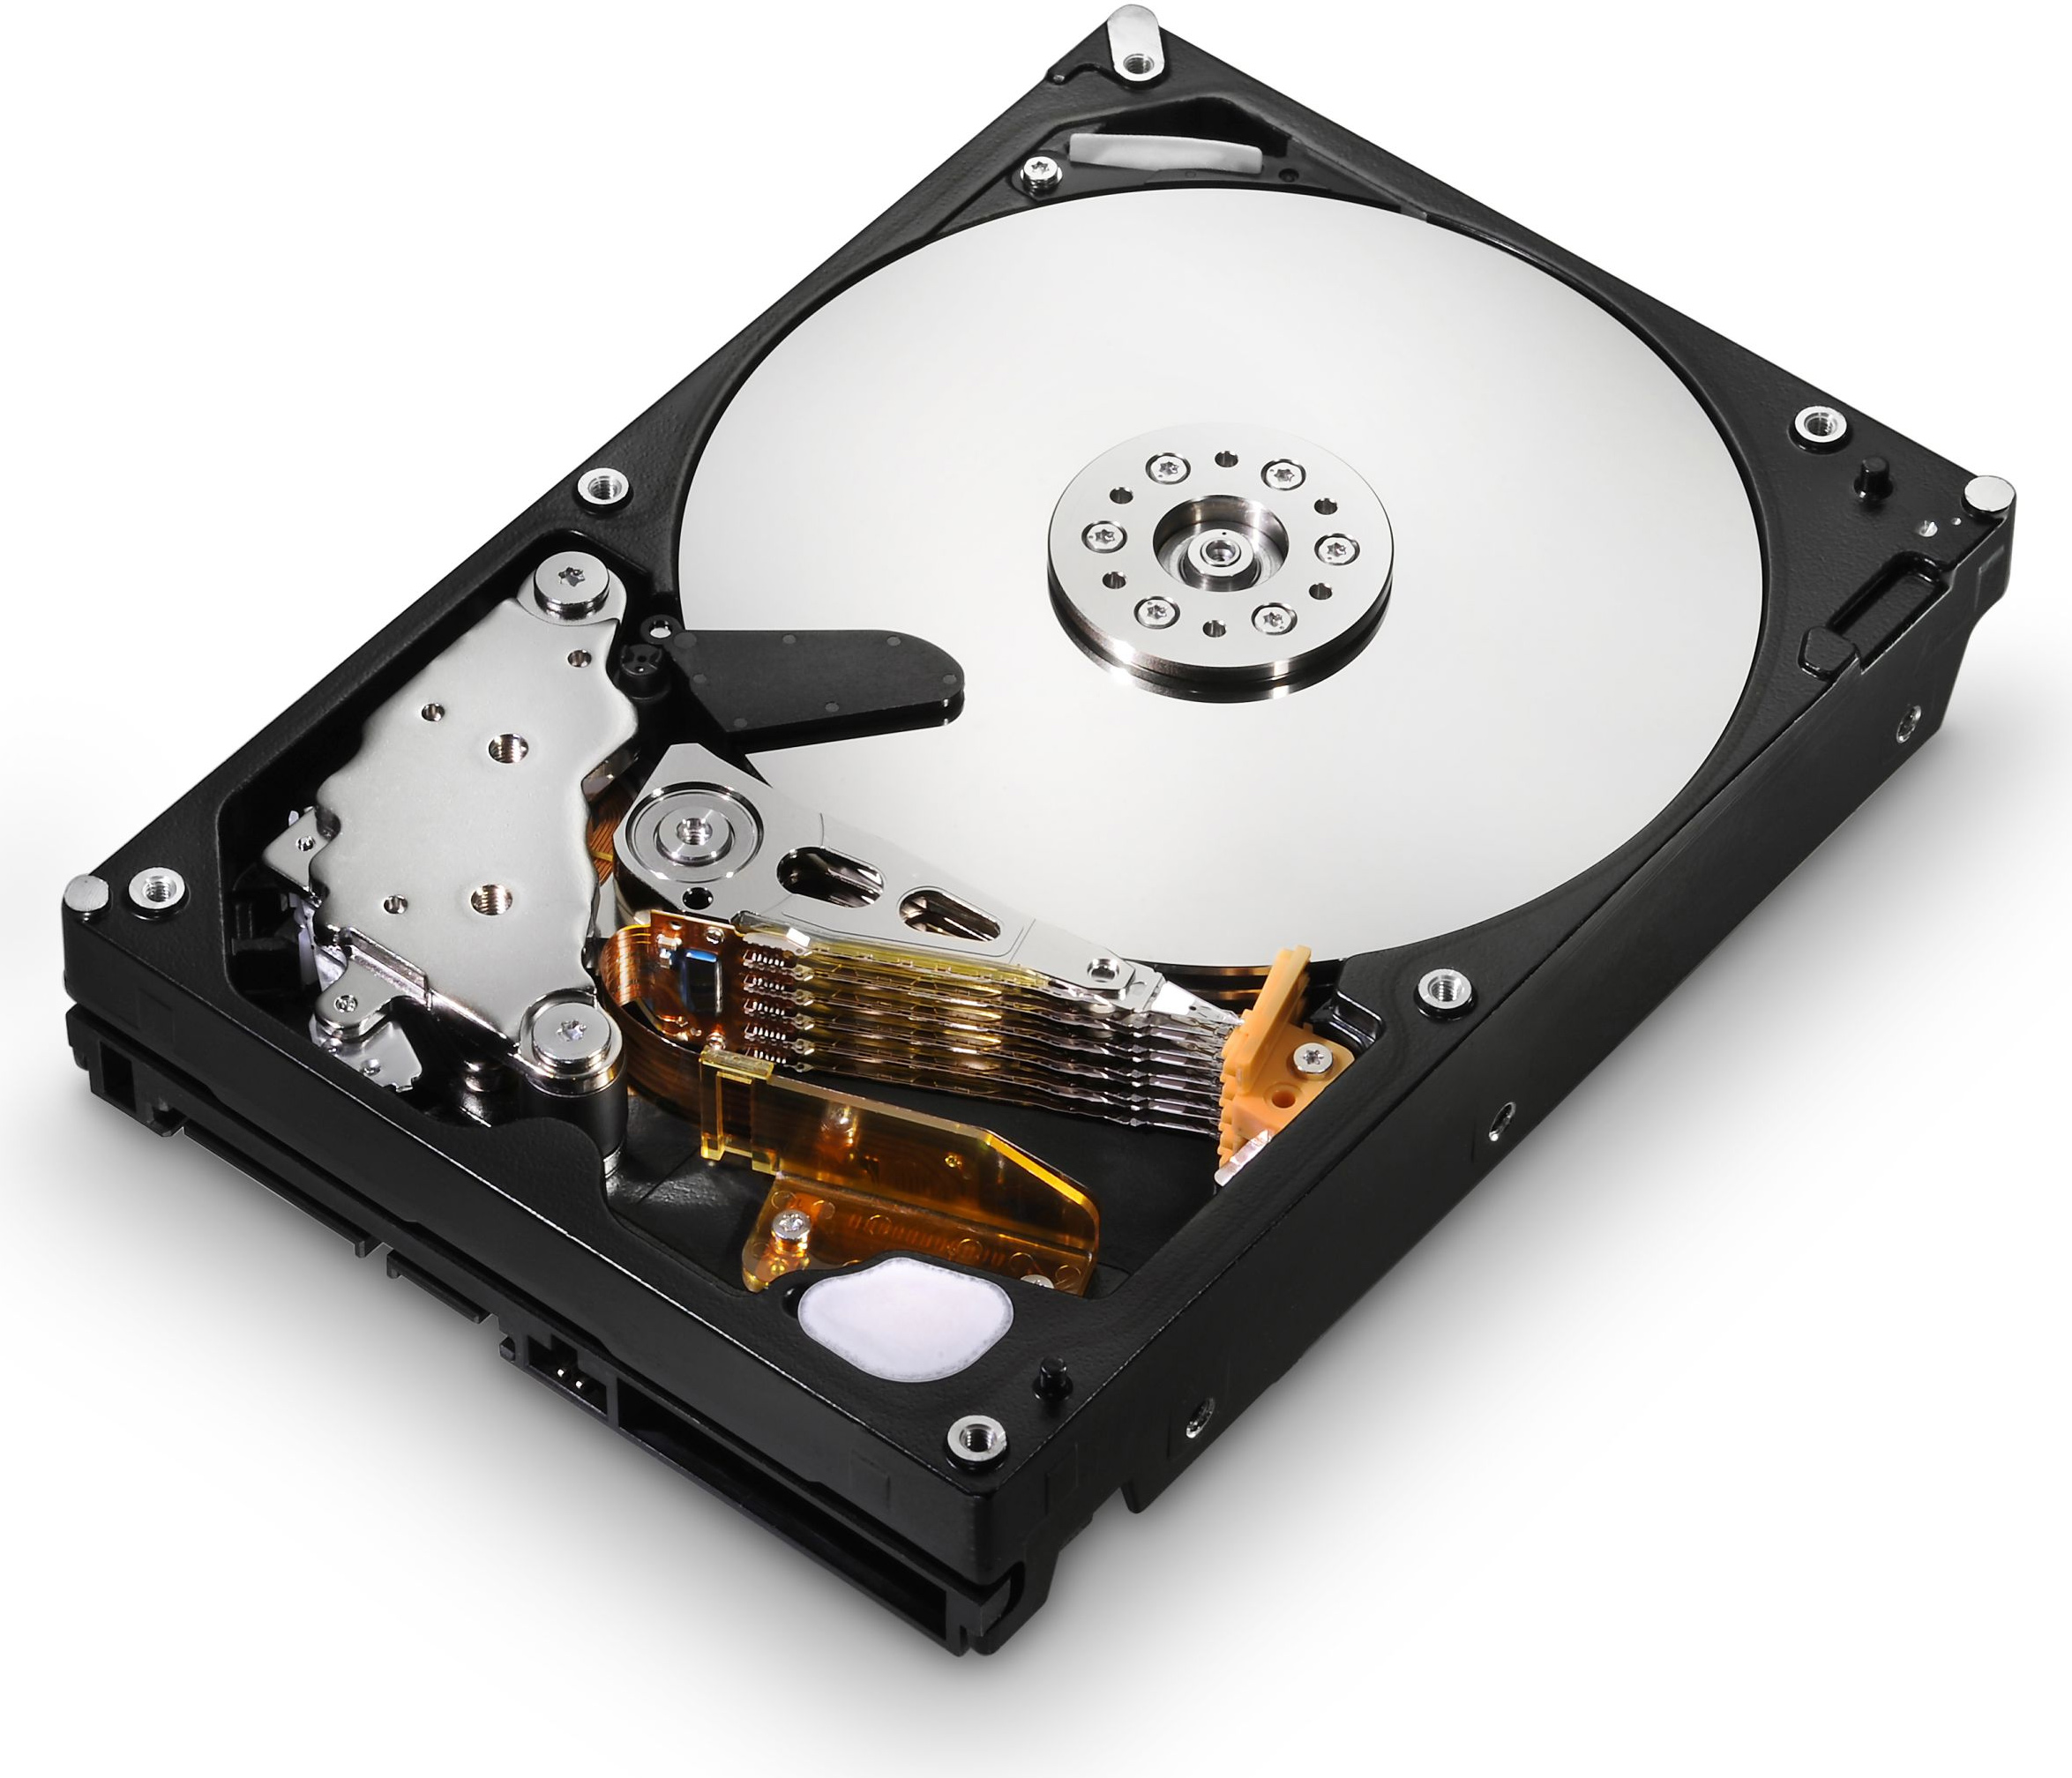
\includegraphics[width=0.2\textwidth]{../figs/HDD.jpg}
	\item RAM (random access memory) is much more expensive
	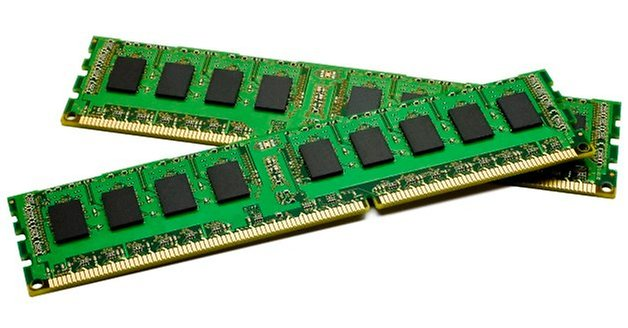
\includegraphics[width=0.2\textwidth]{../figs/RAM.jpg}
	\end{itemize}
	$\rightarrow$ the aspiration is a new type of memory which combinates both positive parts
	
	%\tableofcontents
\end{frame}

%---------------------------------------------------%
\begin{frame}  
	\frametitle{Introduction}
	new approach: \textit{"racetrack memory"}\\ \vspace{5mm}
	$\rightarrow$ consists of a ferromagnetic nanowire\\ \vspace{5mm}
	 (reading and writing by fixed elements)\\ \vspace{5mm}
	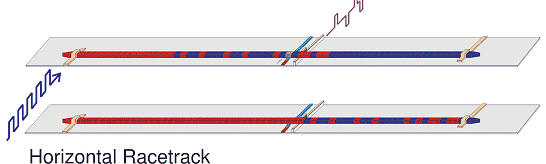
\includegraphics[width=0.8\textwidth]{../figs/horizontal_racetrack.jpg}
\end{frame}

%---------------------------------------------------%
\begin{frame}
	\frametitle{Introduction}
	In the nanowire:
	\begin{itemize}
	\item electrons with spins
	\item align along an external magnetic field 
	\item system of spins with same alignment form $=$ "domain"
	\item "domain-wall between two opposite domains
	\end{itemize}
	\begin{center}
	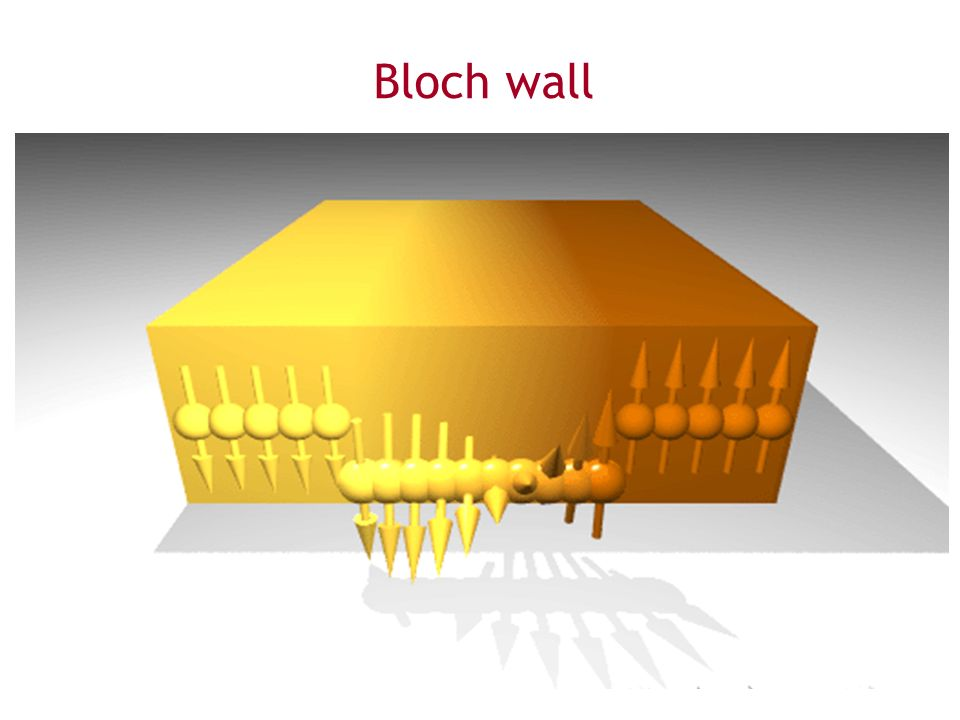
\includegraphics[width=0.6\textwidth]{../figs/bloch_wall.jpg}
	\end{center}
\end{frame}
